%--------------------------------------------------------------------------------
%\documentclass{article}

\documentclass[12pt]{article}
\usepackage[T1]{fontenc} 
\usepackage[bf]{caption}
\usepackage{hyperref}
\usepackage[all]{hypcap}
\usepackage[utf8]{inputenc}
\usepackage{graphicx}
\usepackage[czech, english]{babel}
\selectlanguage{czech}
\usepackage{subfig}                % \subfloat
\usepackage{color}
\usepackage{url}
\inputencoding{utf8}
%\usepackage[bf]{caption2}
\usepackage{hyperref}
\usepackage[all]{hypcap}
\hypersetup{colorlinks=false, linkbordercolor=1 1 1, citebordercolor=1 1 1}
\usepackage[right]{lineno}
\renewcommand\linenumberfont{\normalfont\tiny\color{blue}}


\title{FIT VUT, Počítačové Vidění\\Comic Sans OCR}
\author{Miloslav Číž <xcizmi00>, Daniel Žůrek <xzurek12>}
\date{\today}


%--------------------------------------------------------------------------------

\begin{document}
\selectlanguage{czech}
\maketitle

\section{Zadání a cíle}

Měli jsme implementovat OCR systém za pomoci knihovny OpenCV, přičemž jsme mohli
předpokládat dobrou kvalitu skenovaného textu (málo šumu, dobré zarovnání, bez geometrickcých
deformací apod.). Mohli jsme se rovněž omezit pouze na jeden font. Zadání jsme si upřesnili
následujícím způsobem:

\begin{itemize}
  \item Napsat OCR systém, nabízející několik různých klasifikátorů, v~jazyce C++ za pomoci knihovny OpenCV.
  \item Rozpoznávány budou pouze znaky anglické abecedy, plus pár speciálních znaků:
  \begin{itemize}
    \item malá písmena: "abcdefghijklmnopqrstuvwxyz"
    \item velká písmena: "ABCDEFGHIJKLMNOPQRSTUVWXYZ"
    \item číslice: "0123456789"
    \item speciální znaky: ".,-?"
  \end{itemize}
  \item Rozpoznáván bude pouze font Comic Sans.
\end{itemize}

Cílem bylo vyzkoušet a porovnat různé metody používané pro přepis textu. Cílem nebylo udělat
obecný nebo optimalizovaný OCR systém.

%%%%%%%%%%%%%%%%%%%%%%%%%%%%%%%%%%%%%%%%%%%%%%%%%%%%%%%%%%%%%%%%%%%%%%%%%%%%%%%%%%%%%%%%

\section{Řešení}

Samotný systém se dá rozdělit na dvě části: segmentace a~klasifikace. Museli jsme rovněž vytvořit
dataset pro trénování klasifikátorů.

Práce v~týmu byla rozdělena takto:

\begin{itemize}
  \item Miloslav Číž - dataset, segmentace, MLP, testování, dokumentace 
  \item David Žůrek - KNN
\end{itemize}

\subsection{Dataset}
\label{sec:dataset}

Pro účely testování jsme napsali sedm A4 stran textu v~programu LibreOffice Writer, fontem Comic Sans. Volili jsme
různé velikosti fontu (nejčastěji 12 bodů) a~řádkování. Texty byly většinou zkopírovány z~anglických internetových
stránek jako Wikipedia nebo Reddit. Stránky jsme následně vytiskli a~naskenovali v~rozlišení $2480 \times 3507$ pixelů.
Díle jsme vytvořili zmenšené a~zašuměné verze stránek. Rovněž jsme z~LibreOffice dokumentů extrahovali čistý text
pro pozdější testování kvality přepisu.

Dataset jednotlivých znaků jsme po implementaci segmentace vytvořili segmentací naskenovaných stránek a~ruční
anotací získaných výřezů. Ve výsledku jsme získali cca 3000 anotovaných vzorků. Dataset je dostupný spolu s~kódem a~skenovanými stránkami
na serveru GitHub. \footnote{https://github.com/drummyfish/Comic-Sans-OCR} Pomocí Python skriptu jsme
vytvořili rovněž průměrný obraz každého vzorku pro případné potřeby klasifikátorů.

\begin{figure}[htb]
  \centering
  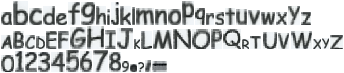
\includegraphics[width=13.5cm,keepaspectratio]{averages.png}
  \caption{průměrné obrazy vzorků znaků}
  \label{fig:avg}
\end{figure}

\subsection{Segmentace}

Segmentace hledá nejprve řádky a~poté jednotlivé znaky v~těchto řádcích, přičemž algoritmus je stejný, jen
se segmentuje podél různých dimenzí. Toto provádí funkce {\tt segmentation\_1d}, která iteruje po
řádcích obrazu a~podle prahu průměrné intenzity vytváří spojité segmenty, které navíc nesmí být příliš malé
ani velké (velké segmenty jsou rozděleny na dva v~polovině).

Každý nalezený výřez je pak ještě před klasifikací upraven tak, že se posunou jeho okraje na přesnou hranici znaku
(funkce {\tt correct\_character\_cutout}).

Mezery se určují pomocí prahové vzdálenosti segmentů (která je zadána relativně k~výšce řádku).

\begin{figure}[htb]
  \centering
  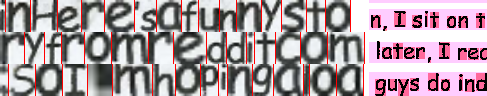
\includegraphics[width=13.5cm,keepaspectratio]{cutouts.png}
  \caption{ukázky segmentace}
\end{figure}

\subsection{Klasifikace}

Pro klasifikaci výřezů jsme využili následujících klasifikátorů:

\begin{itemize}
  \item rastrový klasifikátor \cite{ocr} - Velmi jednoduchý klasifikátor, který porovnává získaný výřez s~průměrným obrazem každého vzorku pomocí korelace. Bere částečně v~potaz i~poměr rozměrů vzorku a~průměrnou intenzitu.
  \item KNN, HoG příznaky - 
  \item MLP - Multilayer perceptron dopředná neuronová síť. Do sítě vstupuje samotný výřez převedený do stupňů šedi a~zmenšený na velikost $10 \times 10$ pixelů. Parametry sítě jsme nalezli experimentálně: 
    \begin{itemize}
      \item vrstvy: 100, 35, 20, 1
      \item backpropagation trénování, maximum 50 iterací, $\epsilon = 10^{-9}$
    \end{itemize}
  \item složený klasifikátor - Využívá všechny výše zmíněné klasifikátory ke hlasování. Není-li při hlasování většina, bere se názor nejúspěšnějšího klasifikátoru (KNN).
\end{itemize}

Natrénované modely klasifikátorů se ukládají do XML souborů, aby trénování neprobíhalo při každém spuštění znovu.

\section{Testování}

Pro testování jsme využili vlastní skenované stránky (viz sekce \ref{sec:dataset}). Metrikou
při porovnání s~referenčními přepisy byla Levenshteinova vzdálenost, tzn. počet editačních kroků. \cite{lev}
Využili jsme vlastní automatizované testy napsané v~jazycích Python a BASH.

Dále jsme porovnávali naše řešení s~kvalitním open-source OCR enginem tesseract. \cite{tess} Tesseract
je velmi komplexní a~je postaven na spoustě pokročilých technologií (baseline fitting, slovníky, neuronové sítě,
dvouprůchodové algoritmy apod.). \cite{tess2}

%%%%%%%%%%%%%%%%%%%%%%%%%%%%%%%%%%%%%%%%%%%%%%%%%%%%%%%%%%%%%%%%%%%%%%%%%%%%%%%%%%%%%%%%

\section{Vyhodnocení}

Tady by mělo být napsané jak to funguje. Protože se jedná o počítačovou grafiku nebo 
vidění, tak by tady měl byt screenshot, ze ktereho bude poznat jak to funguje.
K tomu by měla být idealně tabulka s vyhodnocením jak přesně/rychle to funguje. 

%%%%%%%%%%%%%%%%%%%%%%%%%%%%%%%%%%%%%%%%%%%%%%%%%%%%%%%%%%%%%%%%%%%%%%%%%%%%%%%%%%%%%%%%

\section{Závěr}

Mezi hlavní zjištěné závěry patří:

\begin{itemize}
  \item Zmenšujeme-li výřez znaku na minimální možnou velikost, máme problém s~rozlišování znaků jako ",.'".
  \item Bylo by lepší použít konvoluční neuronovou síť nežli MLP.
  \item Při dobré kvalitě skenů je jednoduchý přístup velmi použitelný.
\end{itemize}

\bibliographystyle{abbrv}
\begin{flushleft}
  \bibliography{project}
\end{flushleft}

%\appendix
%\newpage
%\section{}

\end{document}
